% !TEX encoding = UTF-8
% !TEX TS-program = pdflatex
% !TEX root = ../tesi.tex
% !TEX spellcheck = it-IT

%**************************************************************
\chapter{Il progetto di stage}
\label{cap:descrizione-stage}
%**************************************************************

\section{Pianificazione del lavoro}

Le otto settimane lavorative sono state distribuite in quattro periodi:

\begin{itemize}

\item \textbf{Periodo di apprendimento ed analisi}, nel quale sono entrato in contatto con lo \textit{stack tecnologico} da utilizzare, comprese le tecnologie da integrare, ed ho analizzato nel dettaglio quali fossero i requisiti richiesti dall'applicazione;
\item \textbf{Periodo di progettazione}, nel quale per ogni requisito ho trovato la soluzione adeguata, andando a delineare l'architettura dell'applicazione. In questo periodo affiancato a questa attività ho inoltre sviluppato un prototipo, in modo da poter verificare l'adeguatezza e funzionalità delle soluzioni progettate;
\item \textbf{Periodo di sviluppo e codifica}, nel quale ho realizzato la maggior parte del codice dell'applicazione e implementato tutte le \textit{features};
\item \textbf{Periodo di rifinitura e testing}, nel quale ho testato l'applicazione con altri utenti e in base al feedback ho raffinato ulteriormente il prodotto, andando a risolvere i numerosi \textit{bug} emersi;

\end{itemize}

Di seguito viene riportato il diagramma di Gantt relativo alla pianificazione del lavoro realizzata prima dell'inizio dell'attività di stage:

\begin{figure}[htpd]
\centering
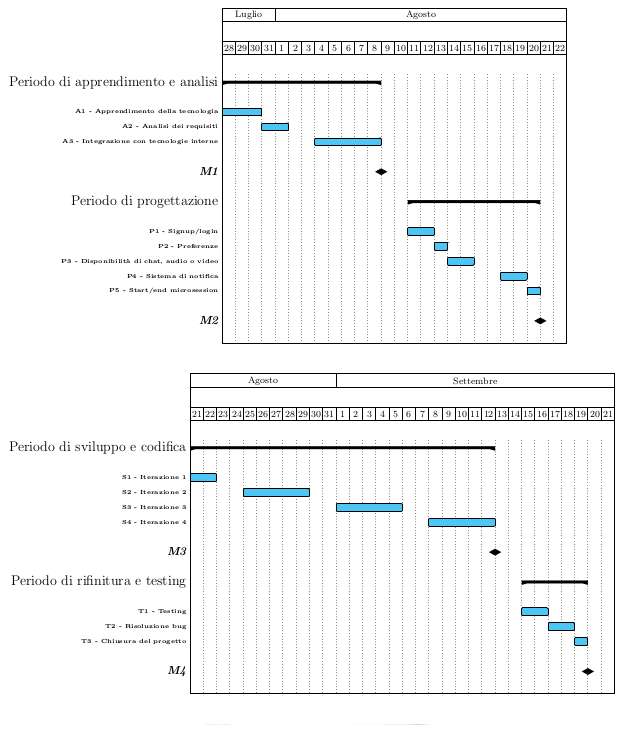
\includegraphics[width=\textwidth]{../immagini/gantt}
\caption{Diagramma di Gantt relativo alla pianificazione del lavoro}  
\end{figure}

\section{Norme, procedure e strumenti}

\subsection*{Strumenti generali}

Per la gestione delle \textit{story} è stato scelto lo strumento \textbf{pivotal tracker}\footnote{\url{https://www.pivotaltracker.com/signin}}, tramite il quale è possibile tener traccia di tutte le story ed avere una panoramica sulle \textit{board}. In particolare è possibile creare progetti condivisi tra più utenti e quindi aver sempre a disposizione il monitoraggio del proprio lavoro e di quello degli altri membri.

\begin{figure}[htpd]
\centering
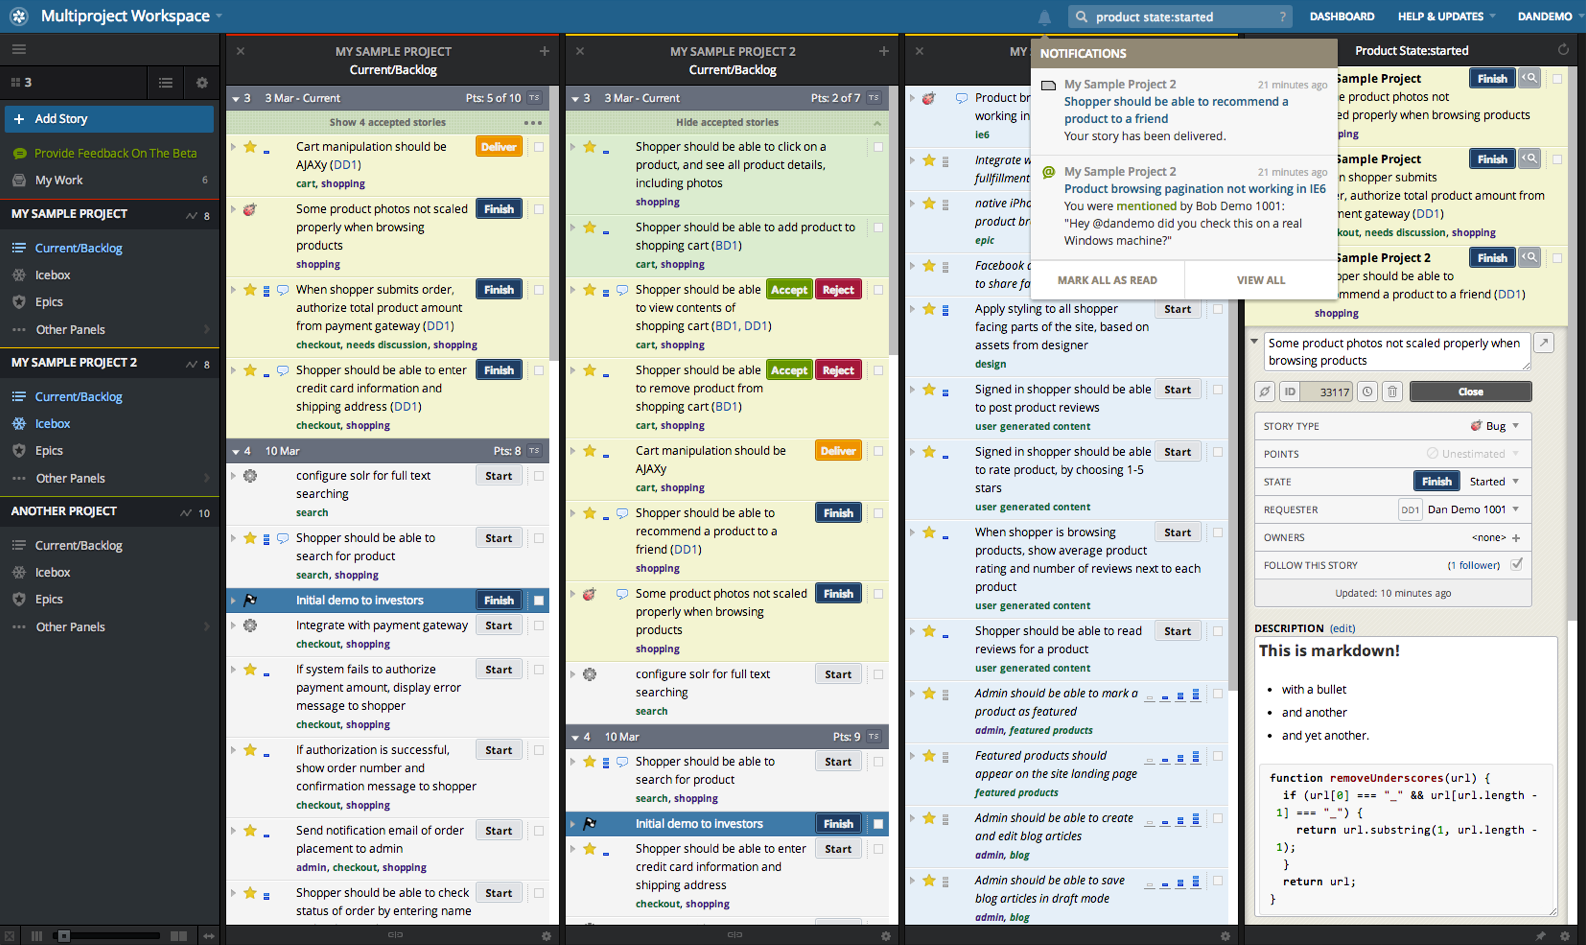
\includegraphics[width=\textwidth]{../immagini/pivotal-tracker}
\caption{Schermata di pivotaltracker}  
\end{figure}

Per la comunicazione interna al \textit{team} è stato scelto l'utilizzo di \textbf{hipchat}\footnote{\url{https://www.hipchat.com/}}, il quale fornisce un sistema di messaggistica istantanea e di video conferenze, in modo analogo a quanto offerto da servizi come \textit{skype} o \textit{google hangout}. Hipchat permette inoltre di creare delle ``stanze'' con più utenti, in modo da poter discutere di un preciso argomento o tema. È altresì possibile marcare i messaggi con degli \gls{hashtag}, in modo da poter gestire al meglio le tematiche. Questo strumento è di fatto fondamentale per poter lavorare da remoto.

\begin{figure}[htpd]
\centering
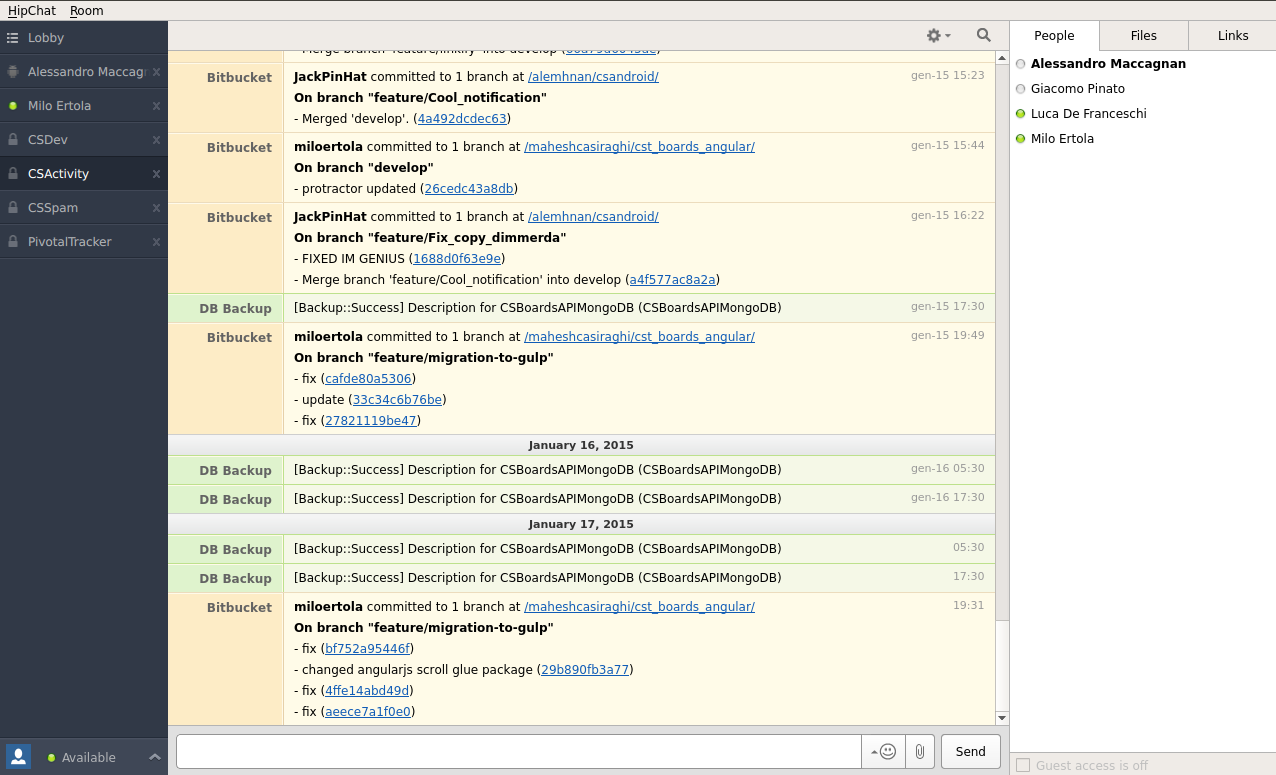
\includegraphics[width=\textwidth]{../immagini/hipchat}
\caption{Schermata di HipChat}  
\end{figure}

Per quanto riguarda la produzione di documenti viene utilizzato lo strumento \textbf{google documents}\footnote{\url{http://www.google.com/docs/about/}}. Questa scelta è dovuta alla estrema facilità di utilizzo e familiarità di tale strumento oltre alla possibilità di condividere documenti in tempo reale ed avere essi disponibili in ogni momento e con ogni piattaforma. Inoltre con google documents è possibile inserire in ogni documento dei \textit{suggerimenti}, che in seguito l'autore o gli autori prenderanno in considerazione.

\subsection*{Formazione e analisi}

All'inizio dell'attività di stage il mio bagaglio tecnico era in linea con l'insegnamento accademico del mio corso di laurea, quindi sostanzialmente avevo buone conoscenze riguardo al linguaggio \textbf{C++}, \textbf{Java}, \textbf{Javascript} e \textbf{PhP}. Inoltre possedevo discrete conoscenze di gestione di database relazionali e documentali, oltre ad una buona preparazione circa lo sviluppo web.

Ciononostante non avevo mai prima di allora sviluppato un'applicazione mobile. Le mie conoscenze in ambito Android erano piuttosto limitate, avevo frequentato alcuni seminari presso l'università e mi ero cimentato per un breve periodo.

A fronte di questa mancanza di conoscenza è stato dunque necessario instanziare un periodo di autoformazione, in modo da entrare in contatto con la tecnologia e poter dunque realizzare l'applicazione. Quest'attività è stata svolta principalmente tramite la lettura e lo studio delle guide Android, messe a disposizione nel sito ufficiale.\footnote{\url{http://developer.android.com/training/index.html}}. Oltre a questo ho consultato le altrettante guide per ciascuna delle tecnologie da integrare all'interno dell'applicazione. Tutti i siti web consultati possono essere trovati in bibliografia. Non ho ritenuto essenziale fornirmi di un libro di testo in quanto le guide e i numerosi esempi disponibili nella rete erano di per sè più che sufficienti.

Per quanto riguarda l'analisi dei requisiti non vi è stata una norma o attività instanziata \textit{ad hoc}, in quanto essa avrebbe rallentato il processo di sviluppo. Non vi è stato inoltre una documentazione e un tracciamento dei requisiti in quanto, essendo che in essi cambiano rapidamente, quest'ultime attività avrebbero portato ad un dispendio di tempo notevole e ad un conseguente rallentamento dello sviluppo. La principale metodologia di supporto all'analisi è stata il semplice \textit{brainstorming}.

\subsection*{Progettazione}

In questo periodo ho iniziato ad ideare l'architettura software dell'applicazione e concorrentemente a sviluppare un \textit{prototipo} secondo i requisiti emersi. Per questo ho installato e configurato l'SDK ufficiale di Android, utilizzando in primo luogo l'\gls{IDE} Eclipse\footnote{\url{https://eclipse.org/home/index.php}}, il quale mette a disposizione un ottimo plugin per la sua integrazione ed è tuttora supportato ed ampiamente usufruito dalla comunità degli sviluppatori. La sua scelta è dovuta inoltre alla familiarità da parte mia con questo strumento, il quale era stato da me utilizzato per progetti precedenti.  

Per la progettazione del layout dell'applicazione ho utilizzato \textbf{lucidchart}\footnote{\url{https://www.lucidchart.com/?utm_expid=39895073-63.LohXHUI7T6yhe2x7Iyjc7Q.0}} come strumento per la realizzazione di \gls{mockup}. Quest'ultimo stumento è stato inoltre utilizzato per la realizzazione dei diagrammi di attività e classi in \gls{UML}. Lucidchart si è rivelato uno strumento molto utile e di facile utilizzo, che permette una gestione sia \textit{online} che \textit{offline} dei diagrammi e permette ad altri utenti di condividere un documento e modificarlo in tempo reale. Quest'ultima caratteristica si è rivelata particolarmente utile nel momento in cui vi era necessità di discutere sulla progettazione. 

\begin{figure}
\begin{minipage}[b]{7cm}
\centering
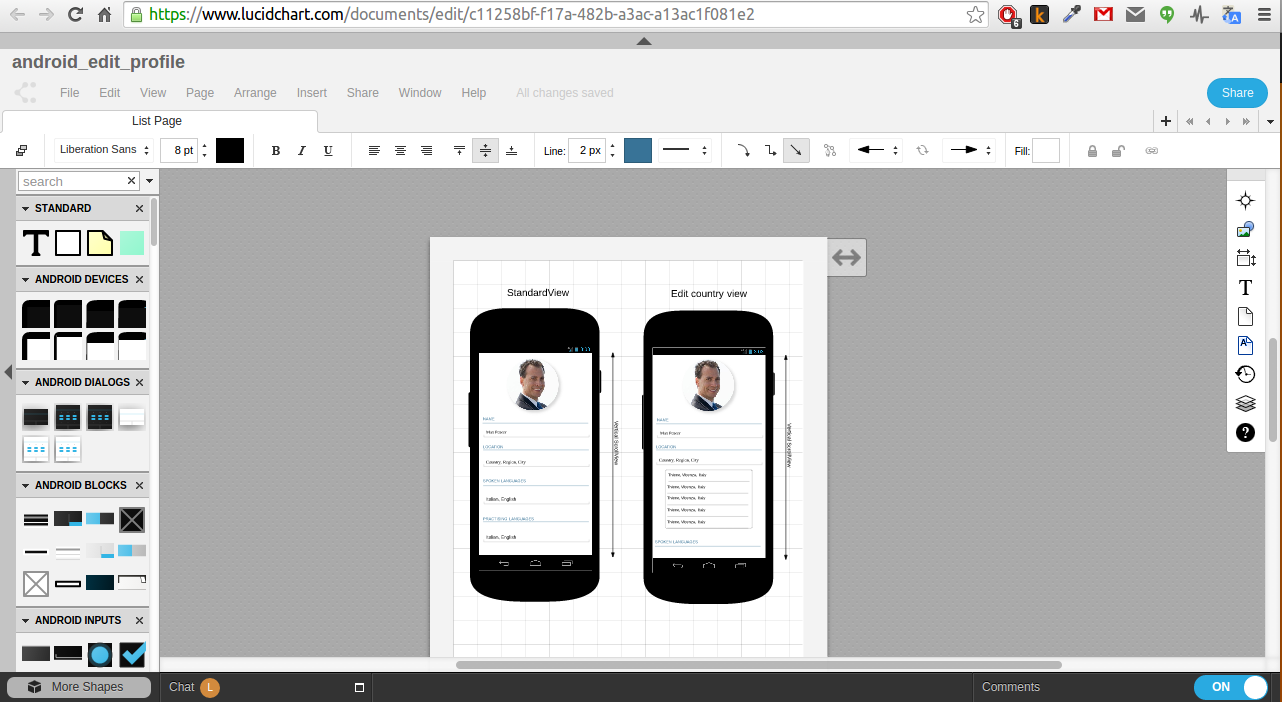
\includegraphics[width=7cm]{../immagini/lucidchart-mockup}
\caption{Lucidchart per la realizzazione di mockup}
\end{minipage}
\ \hspace{2mm} \hspace{3mm} \
\begin{minipage}[b]{7cm}
\centering
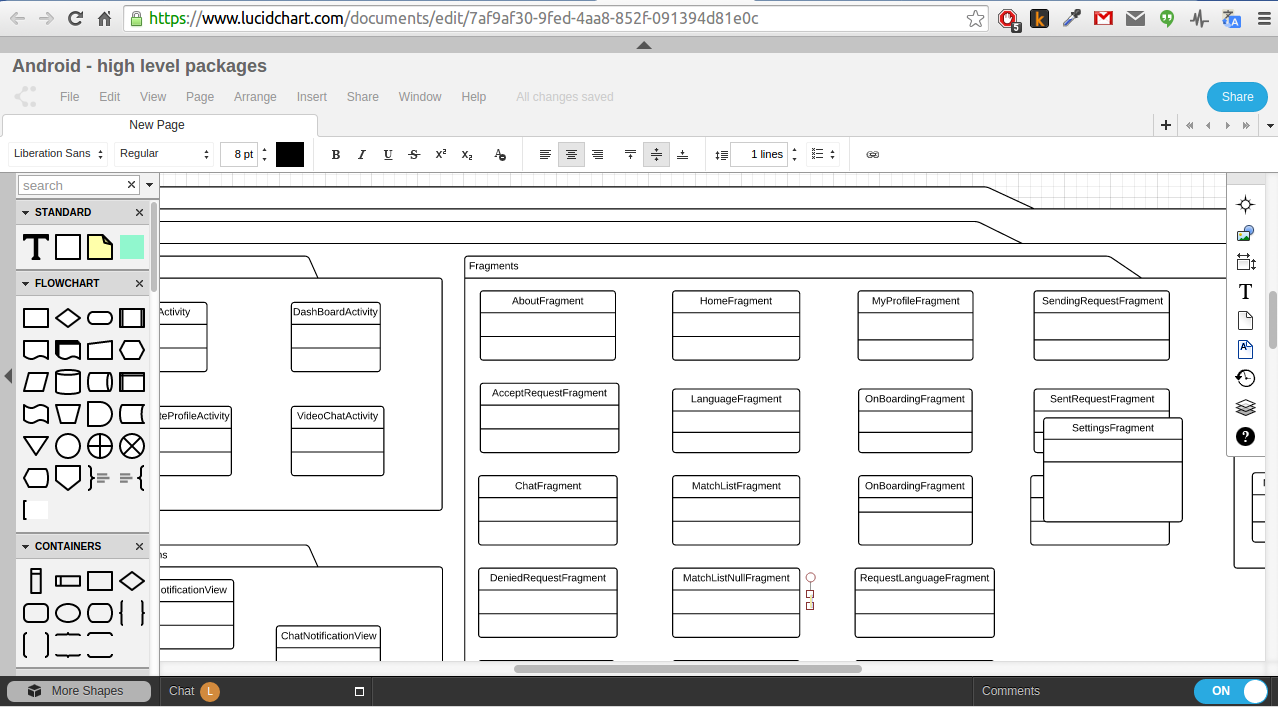
\includegraphics[width=7cm]{../immagini/lucidchart-uml}
\caption{Lucidchart per la realizzazione di diagrammi UML}
\end{minipage}
\end{figure}


\subsection*{Codifica}

In seguito al periodo di progettazione ho deciso, per questioni di efficienza, di abbandonare Eclipse per passare dunque ad \textbf{Android Studio}\footnote{\url{http://developer.android.com/sdk/index.html}}, il quale è sviluppato dall'azienda stessa e può quindi supportare meglio gli ultimi aggiornamenti della piattaforma. Le principali differenze tra i due IDE sono le seguenti:

\begin{itemize}

\item Android Studio utilizza un sistema di compilazione basato su \textbf{gradle}\footnote{\url{https://www.gradle.org/}}, a differenza di Eclipse che utilizza \textbf{ant}\footnote{\url{http://ant.apache.org/}}. Gradle incorpora al suo interno i concetti e la logica di \textit{ant} ed \textbf{apache maven}\footnote{\url{http://maven.apache.org/}}, introducendo inoltre un DSL basato su \textbf{Groovy}\footnote{\url{http://groovy.codehaus.org/}}, che permette la facile codifica di script per l'automatizzazione di processi quali compilazione, verifica o caricamento di file \texttt{.apk} all'interno dello store. Ant, al contrario, si basa su una sintassi in formato XML ed è molto più ``anziano'' rispetto a gradle ma permette anch'esso la codifica di script per l'automatizzazione di processi. Avere a disposizione una serie di processi automatizzati ha come conseguenza un notevole risparmio di tempo, che si traduce in efficienza, oltre che a considerevoli vantaggi in termini di estensibilità e manutenzione del software. La scelta di gradle è dovuta in primo luogo al supporto da parte di Android di questo strumento, il quale viene indicato come \textit{best practice} per il presente e il futuro. Inoltre gradle è risultato per me di più facile utilizzo per la gestione delle dipendenze e per la compilazione, nonchè per la produzione ed esportazione dei file \texttt{.apk};
\item Android Studio offre uno strumento di \gls{refactoring} migliore rispetto ad Eclipse, inoltre il sistema di auto-completamento del codice a mio parere è altresì migliore;
\item La gestione dell'interfaccia grafica è a mio parere migliore in Android Studio rispetto ad Eclipse, le opzioni di personalizzazione sono più vaste e rispondono in modo migliore alle mie esigenze;
\item Se da un lato Eclipse risulta più ``leggero'' in quanto a consumo di risorse, d'altro canto presenta diverse problematiche nell'esecuzione di alcune operazioni, come l'esportazione di file \texttt{.apk}. È capitato più volte infatti che l'IDE terminasse inaspettatmente il suo flusso (\gls{crash}) oppure si bloccasse per un tempo indeterminato (\gls{freeze}). Android Studio da questo punto di vista mi ha garantito maggiore affidabilità. 

\end{itemize}

\begin{figure}[htpd]
\centering
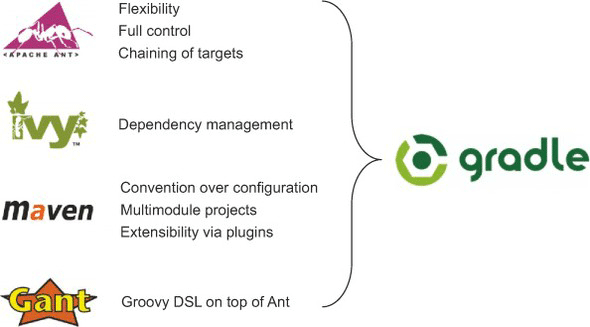
\includegraphics[width=\textwidth/2]{../immagini/gradle}
\caption{Gradle combina tutte le migliori features dagli altri strumenti di sviluppo}  
\end{figure}

\subsection*{Testing}

Il principale strumento utilizzato in fase di verifica è sato \textbf{bugsnag}\footnote{https://bugsnag.com/}, il quale tramite una libreria permette la sua integrazione all'interno di un progetto Android. Il suo utilizzo consiste nella segnalazione e tracciamento di arresti anomali dell'applicazione. Ogniqalvolta all'interno di un'istanza dell'applicazione avviene un arresto anomalo bugsnag automaticamente invia una segnalazione al proprio server, riportando il tipo di errore, dove esso si è verificato e su quale dispositivo. Nella sua pagina web è possibile visualizzare una tabella con il \textit{log} di tutti gli errori, raggruppati per tipologia, e il numero di occorrenze. Questo strumento si è rivelato di estrema importanza per il rilevamento e tracciamento di \textit{bug} all'interno dell'applicazione.

\begin{figure}[htpd]
\centering
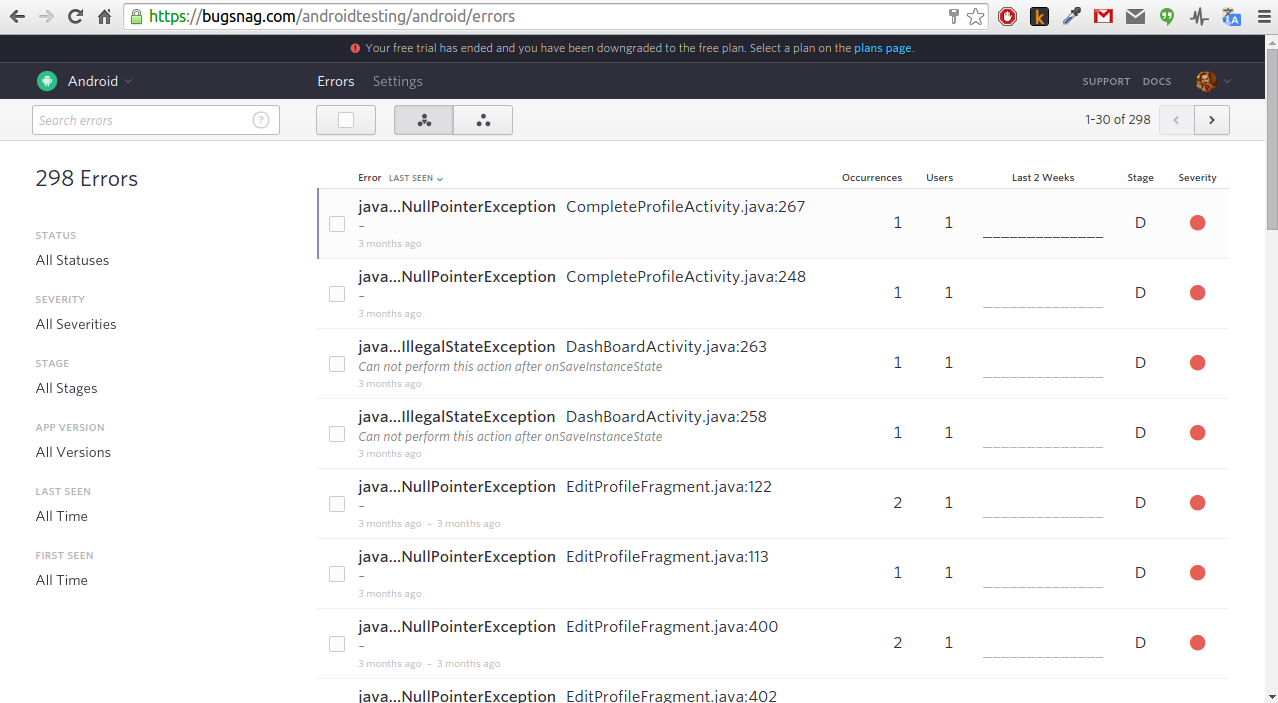
\includegraphics[width=\textwidth]{../immagini/bugsnag}
\caption{Una schermata di bugsnag}  
\end{figure}

\section{Periodo di formazione}

\subsection{Apprendimento della tecnologia}

In questa sezione descriverò come ho appreso la tecnologia di riferimento e attraverso quali processi, approfondendo nel dettaglio alcuni concetti indispensabili e di rilievo. Descriverò la differenza tra le mie conoscenze alla fine di questo periodo e all'inizio, fornendo evidenza di apprendimento.

\subsection{Integrazione con le tecnologie aziendali}

In questa sezione descriverò come, dopo uno studio della tecnologia legata al progetto di stage abbia integrato quest'ultima con le tecnologie già esistenti utilizzate all'interno dell'azienda.

\section{Progettazione}

\subsection{Progettazione del flusso utente}

In questa sezione descriverò la progettazione del flusso utente all'interno dell'applicazione Android, avvalendomi di diagrammi di attività e di flusso.

\subsection{Progettazione del layout}

In questa sezione descriverò la progettazione del layout delle diverse schermate dell'applicazione, giustificando le varie scelte secondo criteri di accessibilità e usabilità.

\subsection{Progettazione architetturale}

In questa sezione descriverò la progettazione dell'architettura software dell'applicazione, andando ad evidenziare la suddivisione in classi e pacchetti, le interazioni di quest'ultimi, le librerie esterne e i design pattern utilizzati; il tutto in relazione con le best-practise indicate dalla comunitò di sviluppatori Android.

\section{Sviluppo e codifica}

In questa sezione descriverò come ho realizzato il codice dell'applicazione aderendo alla progettazione attuata in precedenza.

\section{Rifinitura e testing}

In questa sezione descriverò come a fronte dello sviluppo e codifica dell'applicazione ho proceduto alla sua verifica, istanziando un sistema di bug tracking e testando l'applicazione con utenti reali.

\section{Validazione del prodotto e rilascio}

In questa sezione infine descriverò come a fronte dell'attività di rifinitura è stata istanziata un'attività di validazione mirata a verificare che il prodotto corrispondesse alle aspettative e soddisfasse gli obiettivi preposti. Inoltre descriverò l'attività di rilascio e di pubblicazione di una versione sul play store di Google.